% git_hash=04493d9f, timestamp=2026-07-21 16:46:12 EDT
%%%% Chapter file for Knowledge Representation %%%%
% This chapter file can be compiled standalone or included in the root book.tex

\chapter{Knowledge Representation}
\label{chap:knowledge-representation}

\motto{A machine can only reason about what its representation lets it say.}

% From: book_springer/lectures_source/Lesson04.1_Knowledge_Representation.smd:6 '# Representation as a Foundation for Decisions'
\section{Representation as a Foundation for Decisions}
\label{sec:representation-foundation-decisions}

Every earlier chapter assumed that a decision system has something to reason
over: a set of facts, a causal structure, a distribution to update. This chapter
steps back to ask where that substrate comes from. \emph{Knowledge representation}
(KR) is the discipline of choosing how facts, rules, and relationships get
encoded so that a machine can manipulate them at all, and the choice is not
neutral. A representation that cannot express a distinction cannot reason
about it, no matter how sophisticated the inference procedure built on top of
it. The sections below work through why representation matters, what
formally counts as a KR scheme, the tradeoff between how much a scheme can say
and how efficiently it can be reasoned over, the split between symbolic and
learned representations, and finally how natural language and programming
languages fit, or fail to fit, the same mold

% From: book_springer/lectures_source/Lesson04.1_Knowledge_Representation.smd:8 '* Why Knowledge Representation Matters'
\textbf{Why Knowledge Representation Matters} --- Learning alone is not
enough. A model trained on patient records can predict which disease a
patient likely has, but predicting is not the same as \emph{reasoning}: to
explain that diagnosis to a doctor, in terms the doctor can check and
challenge, the system needs structured knowledge it can manipulate and
inspect, not just a fitted function that emits a label. This is the first
reason KR matters, and it generalizes well past medicine, to any setting
where a machine's output has to survive contact with a human who asks
``why?''

KR also does specific structural work inside an AI system: it bridges
perception and reasoning. Sensors, cameras, logs, and forms all deliver raw
data, which is perception. KR is what turns that raw data into knowledge a
reasoning process can act on, the step that converts a stream of pixels or
numbers into a symbol like \texttt{Patient(P1)} or a probability attached to
a variable a decision procedure can condition on. Without this translation
step, perception and reasoning are two systems that cannot talk to each
other

A third reason is explainability. Once knowledge is represented explicitly,
a system can expose \emph{why} it reached a conclusion, tracing the chain of
facts and rules that produced it, rather than presenting a bare output. This
capability is not a nicety; it is close to mandatory in high-stakes domains
such as healthcare, law, and autonomous systems, where a decision that
cannot be justified is a decision nobody responsible can sign off on

The fourth reason is what makes explicit representation more than a
debugging convenience: it enables what might be called white-box learning.
A robot that plans a route through a warehouse is manipulating abstract
symbolic knowledge about rooms, obstacles, and goals, not raw sensor
readings. A conversational agent that tracks what a user actually wants
across a dialogue is reasoning about intent and context, categories that
only exist because the system represents them. Each of these four
reasons, explaining diagnoses, bridging perception to reasoning,
supporting explainability, and enabling symbolic planning and dialogue,
points at the same underlying fact: the representation is not incidental to
what an AI system can do, it is a precondition for it

% From: book_springer/lectures_source/Lesson04.1_Knowledge_Representation.smd:29 '* What Is Knowledge Representation?'
\textbf{What Is Knowledge Representation?} --- \begin{definition}
  \emph{Knowledge Representation} (KR) is the study of how to formally encode
  information so that machines can reason with it, spanning schemes such as
  rules, logic, ontologies, and semantic networks
\end{definition}
A KR scheme is defined by two things working together. Its \emph{structure}
is how the knowledge is organized, whether as a flat list of facts, a graph
of concepts, or a set of logical formulas. Its \emph{semantics} is what that
organization is taken to mean, the rule that says what a given structure
asserts about the world. Two schemes can share a structure, say, a labeled
graph, and mean entirely different things depending on how edges are
interpreted, which is why structure alone never fully specifies a
representation

KR sits at the heart of AI, and it complements learning-based approaches
rather than competing with them: a learned model can supply the raw
predictions or embeddings, while a KR layer supplies the scaffolding that
lets those outputs be composed, checked, and explained. It serves as the
bridge between perception, which produces data, and reasoning, which
consumes structured knowledge, echoing the point made in the first slide of
this section from a different angle: it is not that KR is one option among
many for building an AI system, it is the layer that makes reasoning
possible in the first place, and it is essential for explainability and
transparency in intelligent systems

Concretely, machines equipped with an explicit knowledge representation can
draw conclusions that were never directly stated but follow logically from
what is stated, perform planning by searching over sequences of actions
expressed in the representation, and answer queries by looking up or
deriving facts from a knowledge base. None of these three capabilities,
drawing conclusions, planning, and answering queries, is available to a
system that only stores raw data without a representation scheme that
defines what that data means and how it combines

% From: book_springer/lectures_source/Lesson04.1_Knowledge_Representation.smd:50 '* Expressiveness vs. Tractability'
\textbf{Expressiveness vs. Tractability} --- \begin{definition}
  The central tradeoff in choosing a knowledge representation pits
  \emph{expressiveness}, the richness of concepts a scheme can capture,
  against \emph{tractability}, whether reasoning over that scheme can be
  performed efficiently
\end{definition}
As a rule, more expressive languages lead to harder computation: the same
features that let a representation say more about the world also give an
inference procedure more structure to search through, and richer structure
tends to blow up the cost of deciding what follows from what. This tradeoff
can be pictured as a curve with expressiveness on one axis and tractability
on the other, sloping downward, so that gains in one dimension come at the
expense of the other, and three representative regimes sit along that
curve. At the tractable, low-expressiveness end sit \emph{atomic}
representations, which treat each state of the world as a single,
indivisible entity: simple to reason over, but limited in what they can
distinguish, as in depth-first search algorithms that treat a chess
position as one opaque state to be searched from rather than a structured
object with parts

In the middle sit \emph{factored} representations, which capture
relationships between variables but stop short of the full structure needed
for complex objects and relations. Propositional logic is the standard
example: in a Minesweeper-style puzzle, the statement that there is a
breeze at cell $(1,2)$ if and only if a pit sits in an adjacent cell is
written
\begin{equation}
  \label{eq:minesweeper-breeze}
  B_{1,2} \Leftrightarrow (P_{1,1} \lor P_{2,2} \lor P_{1,3})\;,
\end{equation}
a factored statement about named variables and their logical relationships,
more expressive than an atomic state description but still not able to
talk about objects, relations between objects, or quantification over
collections of them

At the expressive, less tractable end sit \emph{structured} representations
such as first-order logic, which can state general rules over unboundedly
many objects, at the cost of undecidability in general. The sentence
$\forall x \, \forall y \, Father(x, y) \Rightarrow Parent(x, y)$, read as
``a father of a person is their parent,'' quantifies over every possible
pair of individuals at once, a claim no factored or atomic scheme can even
express, let alone reason over efficiently. The key insight this tradeoff
forces is that choosing a representation is not a question with one right
answer; it depends on the application, on how much of the tradeoff's
expressiveness a task genuinely needs against how much tractability it can
afford to give up

% From: book_springer/lectures_source/Lesson04.1_Knowledge_Representation.smd:126 '* Symbolic vs. Sub-symbolic Representation'
\textbf{Symbolic vs. Sub-symbolic Representation} --- \emph{Symbolic KR} uses
discrete, human-readable symbols, the kind found in logic and knowledge
graphs. Its chief virtue is interpretability: a symbolic fact like
\texttt{Parent(Alice, Bob)} means exactly what it says, which makes symbolic
schemes well suited to rule-based reasoning where every step can be
inspected. Their weakness is the mirror image of that strength: symbolic
representations struggle with ambiguity, because a discrete symbol either
applies or it does not, with no native way to express that a concept
applies partially or uncertainly

\emph{Sub-symbolic KR} takes the opposite approach, using learned,
distributed representations such as vector embeddings, where a concept is
spread across many continuous-valued dimensions rather than pinned to one
discrete token. This buys graceful handling of similarity and ambiguity,
since nearby vectors can represent related concepts, but it costs
transparency: a 300-dimensional embedding does not carry a legible label
for what it means, and extracting a human-readable justification from it
is far harder than reading a symbolic rule

Figure~\ref{fig:symbolic-vs-subsymbolic} contrasts the two: symbolic
representation organizes knowledge as discrete, labeled structure, while
sub-symbolic representation organizes it as a continuous space where
meaning is implicit in position and distance rather than explicit in a
label. \emph{Neuro-symbolic KR} sits between the two, blending discrete
structure with learned representations to reason over learned concepts
using structured logic, keeping the interpretability of symbols for the
parts of a system that need to be checked and explained while keeping the
flexibility of learned representations for the parts that need to
generalize from data

% rendered_image:begin
% filename: msml610/lectures_source/figures/L03.symbolic_vs_subsymbolic.png
% label: fig:symbolic-vs-subsymbolic
% caption: Symbolic representation encodes knowledge as discrete, labeled
%          structure; sub-symbolic representation encodes it as a
%          continuous, learned space.
% rendered_image:end
\begin{figure}[!t]
  \centering
  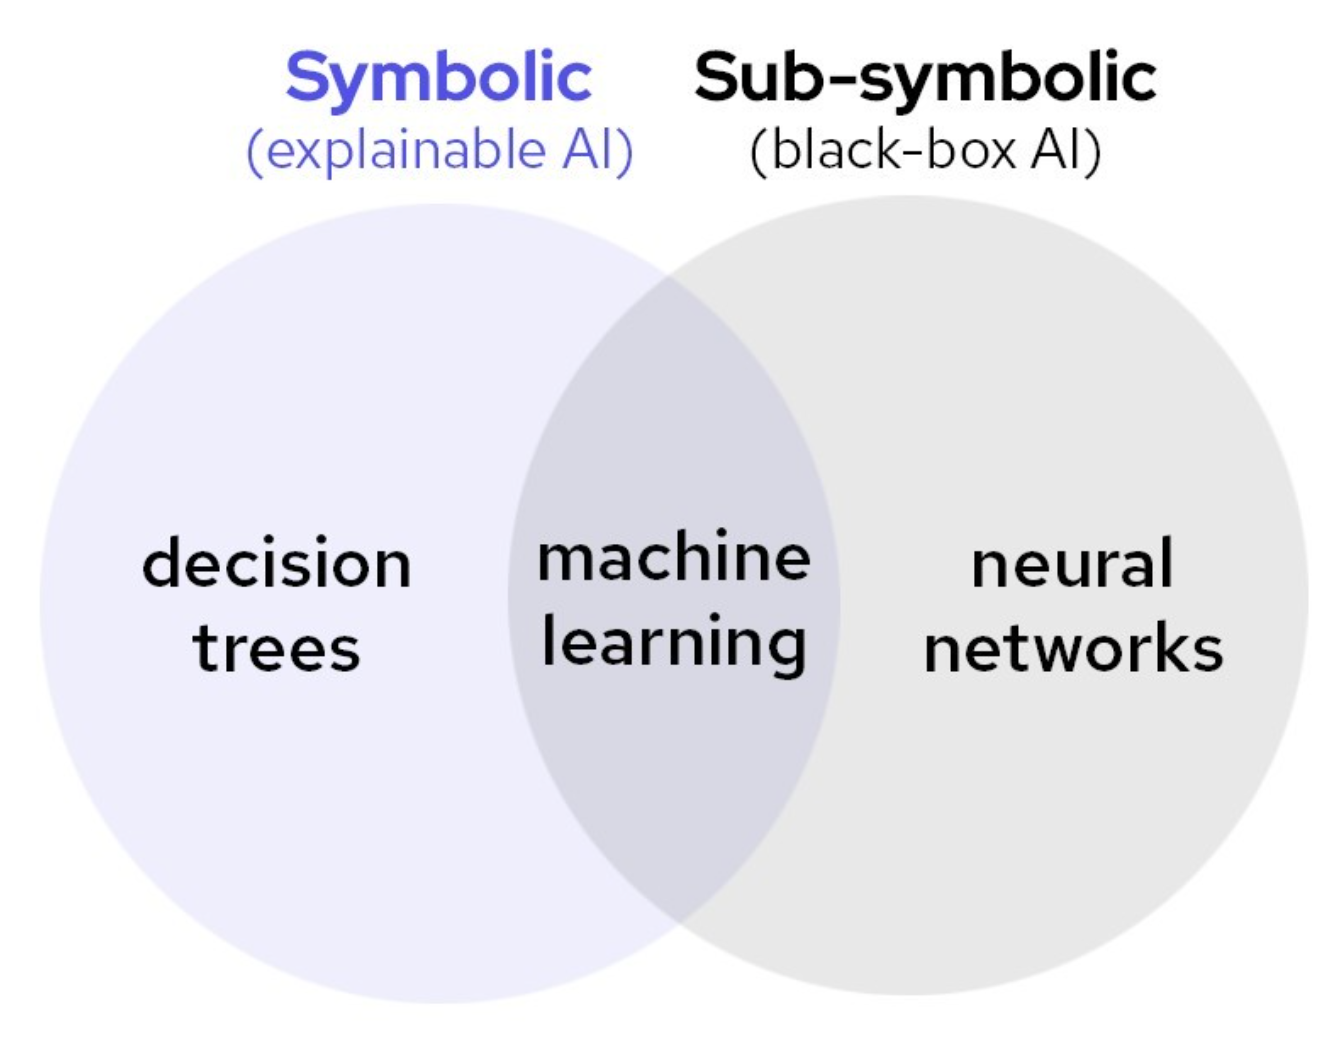
\includegraphics[width=8cm]{../../msml610/lectures_source/figures/L03.symbolic_vs_subsymbolic.png}
  \caption{Symbolic representation encodes knowledge as discrete, labeled
  structure; sub-symbolic representation encodes it as a continuous, learned
  space.}
  \label{fig:symbolic-vs-subsymbolic}
\end{figure}

% From: book_springer/lectures_source/Lesson04.1_Knowledge_Representation.smd:153 '* Neuro-symbolic Approach: Conceptual Spaces'
\textbf{Neuro-symbolic Approach: Conceptual Spaces} --- \emph{Conceptual
spaces} are a neuro-symbolic framework for representing knowledge using
geometric structure rather than discrete symbols alone. Each dimension of
the space corresponds to an interpretable feature, similarity between
objects is modeled as spatial distance rather than as a match or mismatch
between symbols, and a \emph{concept} is not a single point but a region
carved out of this multidimensional space

This geometric framing buys something purely symbolic systems cannot offer
cheaply: a natural way to model similarity and vagueness. A purely symbolic
system represents \texttt{Car} and \texttt{Bicycle} as unrelated discrete
symbols with no structure connecting them, so any claim about how similar
the two are has to be added separately, as an extra fact bolted onto the
representation. A conceptual space, by contrast, places both concepts
somewhere along shared, interpretable dimensions, so the degree of
similarity falls directly out of geometric distance rather than needing to
be stated as an independent axiom

Figure~\ref{fig:conceptual-spaces} works through this with a concrete
example: a conceptual space of transportation methods, organized along two
dimensions, environmental friendliness and technological advancement. Wooden
transportation occupies one region of this space, vehicles occupy a second,
larger region, and advanced vehicles form a nested subset within the
vehicle region, sitting further along the technological-advancement axis.
Nothing about this structure needed to be declared as an explicit rule; the
containment relationships, wooden transportation as a distinct region,
vehicles as a broader category, advanced vehicles as a refinement of it,
emerge from how the regions are positioned and shaped in the space, which is
exactly the kind of graded, geometric structure that a purely symbolic
scheme has no native mechanism for expressing

% rendered_image:begin
% filename: msml610/lectures_source/figures/L03.conceptual_spaces.png
% label: fig:conceptual-spaces
% caption: A conceptual space for transportation methods, with concepts as
%          regions along interpretable dimensions rather than discrete
%          symbols.
% rendered_image:end
\begin{figure}[!t]
  \centering
  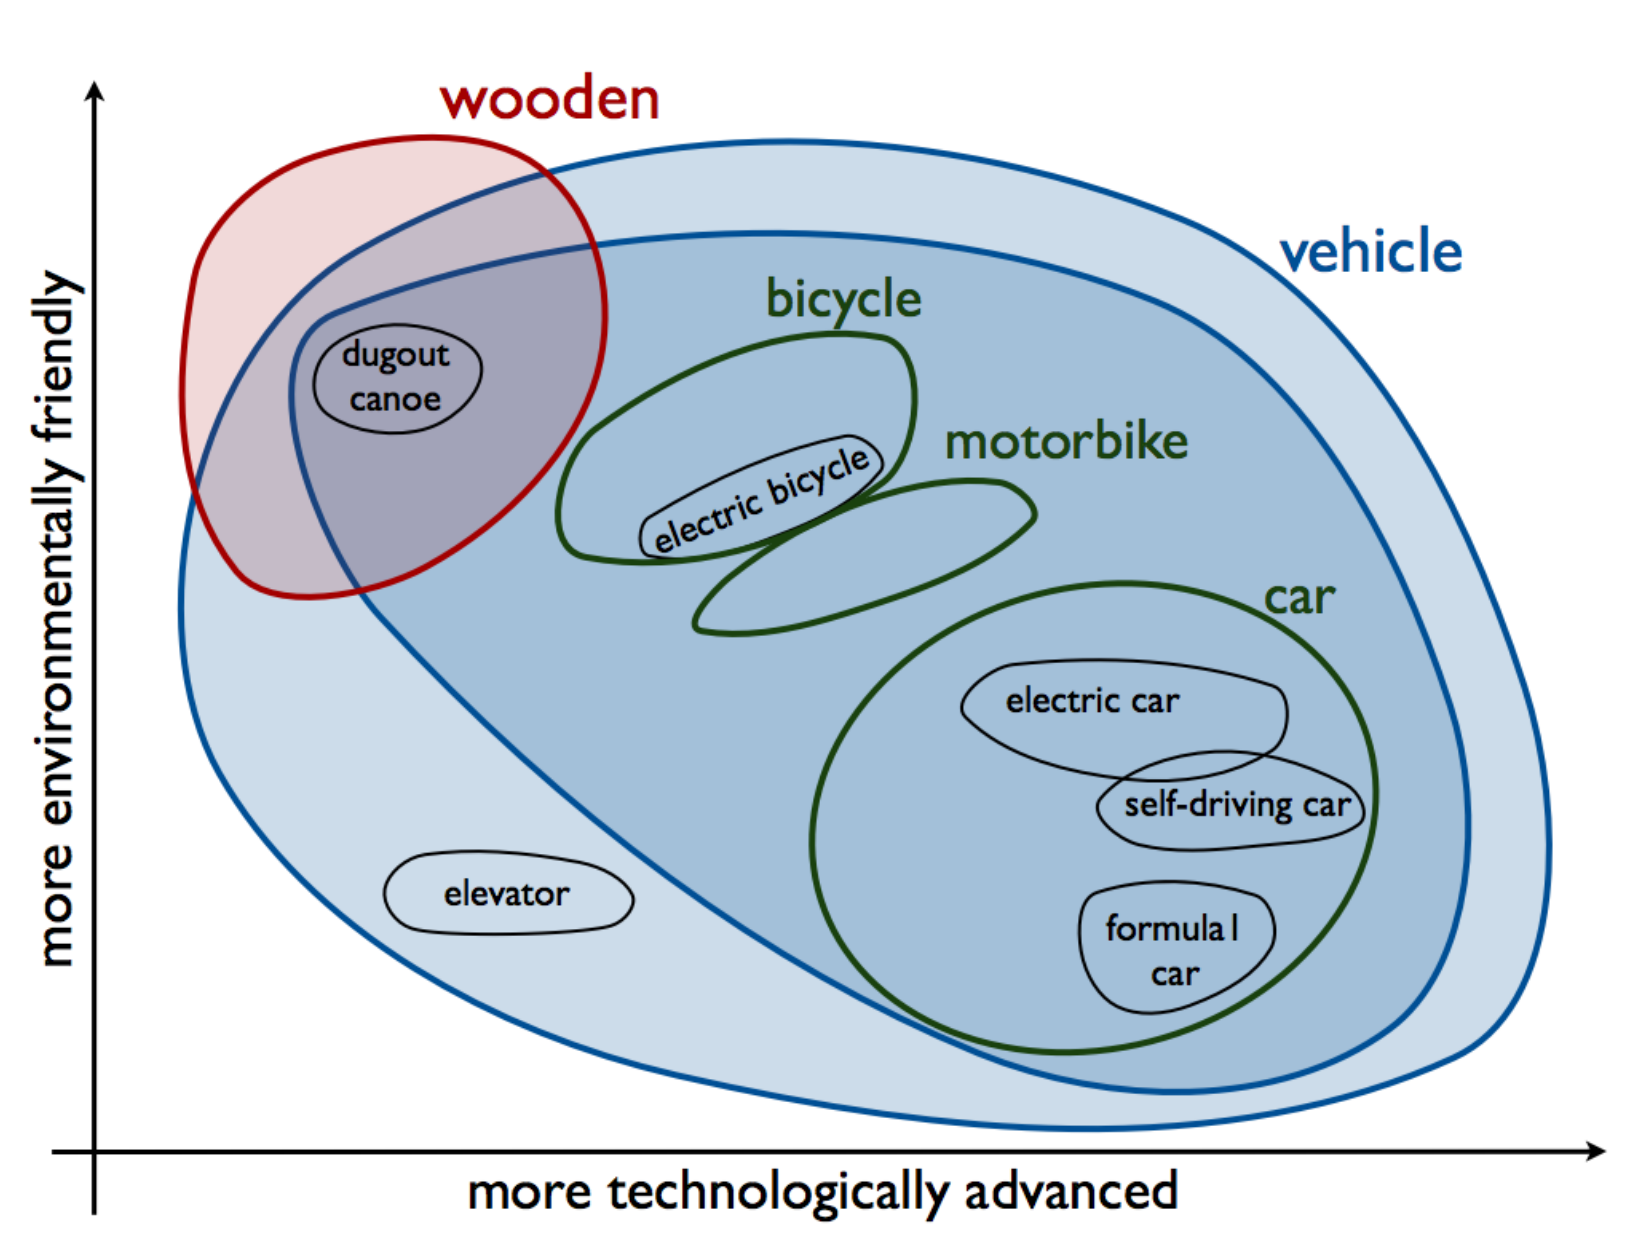
\includegraphics[width=8cm]{../../msml610/lectures_source/figures/L03.conceptual_spaces.png}
  \caption{A conceptual space for transportation methods, with concepts
  represented as regions along interpretable dimensions rather than as
  discrete symbols.}
  \label{fig:conceptual-spaces}
\end{figure}

% From: book_springer/lectures_source/Lesson04.1_Knowledge_Representation.smd:184 '* Procedural vs. Declarative Representation'
\textbf{Procedural vs. Declarative Representation} --- The \emph{procedural
approach} to representing knowledge focuses on \emph{how} a task is done: it
encodes the desired behavior directly into a program, step by step. A robot
programmed with a specific sequence of moves to navigate a maze is a
procedural representation of that navigation task, since the knowledge
\emph{is} the sequence of steps, with no separation between what to
achieve and how to achieve it

The \emph{declarative approach} inverts this: it specifies \emph{what} the
goal is, not \emph{how} to reach it. A declarative representation describes
relationships between actions and goals and leaves the work of finding a
solution to a separate search or inference process. Describing the goal as
``reach the exit of the maze,'' without saying which moves get there, and
letting the robot's planner find a path is a declarative representation of
the same task the procedural example encoded directly

The comparison between the two is a straightforward tradeoff: the
procedural approach offers more direct control over exactly how a task is
carried out but less flexibility, since changing the goal usually means
rewriting the steps; the declarative approach offers more abstraction and is
easier to modify or extend, since changing the goal is a matter of changing
a description rather than a procedure, but it depends on a solver capable
of turning that description into action

Many successful AI systems do not pick one approach over the other; they
use a hybrid, where declarative knowledge is compiled into procedural code
before execution. A planner that takes a declarative goal and generates a
concrete sequence of actions, a plan, is exactly this hybrid pattern in
action: the goal is declared, the mechanism for reaching it is generated
procedurally, and the two representational styles end up working together
rather than in competition

% From: book_springer/lectures_source/Lesson04.1_Knowledge_Representation.smd:207 '* Natural Language as a Representation'
\textbf{Natural Language as a Representation} --- Natural languages such as
English or Italian are a representation scheme humans use constantly, and
they have three properties that make them a poor fit for the kind of formal
reasoning the rest of this chapter builds toward. They are \emph{expressive},
serving primarily as a medium for communication between people rather than
as a representation optimized for machine inference. They are
\emph{ambiguous}: the same word, ``spring,'' can mean a season or a coiled
piece of metal, and nothing in the word itself disambiguates which sense is
meant. And they are \emph{context-dependent}, since the meaning of an
utterance depends on the sentence and situation surrounding it, as with the
single word ``Look!'', whose meaning shifts entirely depending on what is
being pointed at and why

Natural language's influence runs deeper than surface ambiguity, a point
captured by the \emph{Sapir-Whorf hypothesis}: the language a person speaks
shapes how they perceive, think about, and experience the world, and this
shaping happens even through grammatical features that look arbitrary, such
as the gendering of nouns in some languages and not others. If the
hypothesis is right, the representation is not a neutral conduit for
thought; it actively constrains what kinds of thoughts are easy or hard to
have

The clearest illustrations of this constraint come from what languages do
and do not lexicalize. Some languages lack dedicated words for concepts
that other languages express easily, such as certain notions of direction,
while others have many distinct words for a single concept English
collapses into one, as with Arctic languages that distinguish fresh snow
from hard snow with separate terms where English has only ``snow.''
Orwell's invented Newspeak in \emph{1984} pushes this to its logical
extreme as a work of fiction: a language engineered so that certain
concepts, and the thoughts built from them, become literally
unrepresentable to anyone who only has Newspeak's vocabulary to think in

% From: book_springer/lectures_source/Lesson04.1_Knowledge_Representation.smd:231 '* Programming Languages as a Representation'
\textbf{Programming Languages as a Representation} --- A \emph{programming
language} such as \texttt{C++} or \texttt{Python} is itself a formal,
procedural representation scheme: \emph{data structures} represent facts
about the world, and \emph{code} updates those data structures in whatever
way the programmer has decided fits the domain. This makes programming
languages powerful, general-purpose tools, but it also exposes two specific
limitations relative to the KR schemes this chapter is building toward

The first limitation is that programming languages provide no general
mechanism for deriving facts from other facts. Code updates a data
structure according to logic the programmer wrote by hand, based on the
programmer's own domain knowledge, rather than through a domain-independent
inference procedure that could derive new facts from old ones automatically.
The second limitation is expressiveness for partial information: a variable
in a typical programming language holds a single concrete value, or is
undefined, with no built-in way to represent that a fact is only partially
known or to quantify the uncertainty in it. A programming language has no
natural way to encode a statement like ``a white knight is in \texttt{b1}
or in \texttt{f6}'', a genuinely partial piece of information that neither
commits to one square nor leaves the variable completely unset

\emph{Declarative languages} are built to close exactly this gap by keeping
knowledge and inference separate rather than fusing them the way procedural
code does. The \emph{knowledge} component represents the domain-specific
problem, and its meaning is compositional, meaning the meaning of a whole
sentence is built systematically from the meaning of its parts, rather than
handled by ad hoc code. The \emph{inference} component is domain
independent: the same inference procedure, whether it is resolution in
propositional logic or unification in first-order logic, works across any
domain expressed in the language, which is precisely the general mechanism
for deriving facts from facts that a conventional programming language
lacks

% From: book_springer/lectures_source/Lesson04.1_Knowledge_Representation.smd:256 '# Formal Knowledge Representation'
\section{Formal Knowledge Representation}
\label{sec:formal-knowledge-representation}

The previous section established why representation matters and surveyed
the informal spectrum from procedural code to natural language. This
section turns to the formal end of that spectrum: logic-based schemes
designed specifically so that a machine can derive new facts from old ones
through a domain-independent inference procedure. It starts with
propositional logic's syntax and semantics, extends to the quantifiers that
give first-order logic its extra reach, formalizes what it means for one
statement to follow logically from another, and then examines two ways
classical logic's assumptions break down in practice, non-monotonic
reasoning and the closed- versus open-world distinction, before closing
with a framework for learning logical rules directly from examples

% From: book_springer/lectures_source/Lesson04.1_Knowledge_Representation.smd:258 '* Propositional Logic: Syntax and Semantics'
\textbf{Propositional Logic: Syntax and Semantics} --- \begin{definition}
  \emph{Propositional logic} is a formal system for reasoning about
  statements that can be true or false, defined by a \emph{syntax}, which
  fixes the allowable sentences, and a \emph{semantics}, which fixes how
  the truth of a sentence is determined
\end{definition}
The syntax of propositional logic consists of proposition symbols and
logical connectives, so that a sentence such as $P \land Q$ is well formed
because it combines two proposition symbols with a valid connective. The
semantics is the separate question of how the truth of a complex sentence
is evaluated once the truth of its parts is known, typically through truth
tables or deduction rules: if $P$ is true and $Q$ is false, then $P \land
Q$ evaluates to false, regardless of what $P$ and $Q$ actually stand for in
the world

This formal machinery is not merely academic; it underlies several working
technologies. \emph{SAT solvers} are tools for determining whether a
propositional logic formula can be satisfied by some assignment of truth
values, and they are used directly in hardware verification and scheduling
problems, where a design constraint or a scheduling requirement can be
encoded as a formula whose satisfiability answers a concrete engineering
question. \emph{Expert systems} use logic rules to mimic human
decision-making, as in medical diagnosis systems that encode a physician's
if-then knowledge directly as propositional rules. \emph{Rule-based agents}
operate on a set of predefined rules built from this same logical
substrate, as in automated customer service chatbots that route a query
based on which rule's conditions the query satisfies

% From: book_springer/lectures_source/Lesson04.1_Knowledge_Representation.smd:284 '* First-Order Logic: Quantifiers and Inference'
\textbf{First-Order Logic: Quantifiers and Inference} --- Propositional
logic can only talk about named statements one at a time; \emph{quantifiers}
are what let first-order logic express properties of entire collections of
objects at once, instead of enumerating every object by name the way
propositional logic is forced to

The \emph{universal quantifier}, written $\forall x\, P(x)$, makes a
statement about \emph{every} object in the domain: the sentence is true
exactly when $P(x)$ is true for all values of $x$. The \emph{existential
quantifier}, written $\exists x\, P(x)$, makes a weaker claim, that
\emph{some} object, without naming which one, satisfies the property: the
sentence is true as soon as $P(x)$ is true for at least one $x$. These two
quantifiers are what give first-order logic the reach that the earlier
Minesweeper example, restricted to named cells, could never have on its
own

Within a quantified sentence, a variable is either \emph{bound} by a
quantifier or \emph{free}, unbound, and only bound variables have a fixed
logical status independent of context. The sentence $\forall x\,
(Cat(x) \rightarrow Mammal(x))$ binds $x$ under the universal quantifier
and asserts, for every object in the domain, that being a cat implies being
a mammal, a single sentence that stands in for an unboundedly large
conjunction of statements about individual cats, which is exactly the
expressive power that atomic and factored representations, discussed
earlier in this chapter, are structurally unable to provide

% From: book_springer/lectures_source/Lesson04.1_Knowledge_Representation.smd:302 '* Logical Entailment and Inference'
\textbf{Logical Entailment and Inference} --- \begin{definition}
  \emph{Logical entailment} between sentences is the fact that a sentence
  follows logically from another sentence in a knowledge base. ``$\alpha$
  entails $\beta$'', written $\alpha \models \beta$, holds by definition
  exactly when every model in which $\alpha$ is true is also a model in
  which $\beta$ is true, equivalently $M(\alpha) \subseteq M(\beta)$
\end{definition}
Two examples make the definition concrete. In a small ``rain and wet
ground'' world, the sentence $\alpha$: ``$Rain = T, WetGround = T$'' entails
$\beta$: ``$Rain \implies WetGround$''. If it is a fact that it is raining
and the ground is wet, then the conditional rule that rain implies a wet
ground must be true, at least in this particular world; the specific,
concrete fact supports the general conditional rule because every model
consistent with the specific fact is automatically a model in which the
rule holds

A second, purely algebraic example strips away any appeal to intuition
about rain: in a world where $\alpha$ is ``$x = 0$'' and $\beta$ is
``$x \cdot y = 0$'', $\alpha$ entails $\beta$ because in any model where
$x = 0$ holds, $x \cdot y = 0$ holds as well, regardless of what value $y$
happens to take. The entailment goes through purely from the structure of
the two sentences, with no need for the ``sitting table'' world to have any
particular character beyond satisfying $\alpha$

The intuition worth keeping from both examples is that entailment is not a
proof procedure; it is a semantic relationship that ``preserves truth''
across every model consistent with the premise, which makes it a
constraint on what it is consistent to believe. If a knowledge base is
believed, every sentence that base entails must be believed as well, not
because a specific derivation was carried out, but because disbelieving an
entailed sentence while believing the premises that entail it is, by the
definition above, an inconsistent position to hold

% From: book_springer/lectures_source/Lesson04.1_Knowledge_Representation.smd:330 '* Non-Monotonic Logic and Default Reasoning'
\textbf{Non-Monotonic Logic and Default Reasoning} --- \emph{Non-monotonic
logic} is a logic in which adding new information can invalidate
conclusions that were previously derived, a property that separates it
sharply from classical logic. In classical logic, once a conclusion is
proven it remains true no matter what further information arrives; in
non-monotonic logic, conclusions are explicitly allowed to change as new
facts are learned, which is closer to how everyday reasoning actually
behaves

The standard illustration is Tweety the bird. Starting from a knowledge
base containing ``birds typically fly'' and ``Tweety is a bird,'' the
natural conclusion is ``Tweety can fly.'' Adding the new facts ``Tweety is
a penguin'' and ``penguins cannot fly'' does not just add information
alongside the old conclusion, it overturns it, producing the revised
conclusion ``Tweety cannot fly.'' A classical, monotonic logic has no way
to represent this kind of retraction, since a once-derived conclusion is
permanent by construction

This matters because real-world reasoning is built on incomplete or
evolving knowledge almost by default: an agent rarely has the complete
picture up front and has to act on defaults that later facts can override.
Non-monotonic logic gives a system the flexibility to reason under exactly
this condition, drawing a reasonable conclusion from typical-case defaults
while remaining able to revise that conclusion cleanly the moment an
exception, like Tweety turning out to be a penguin, is learned

% From: book_springer/lectures_source/Lesson04.1_Knowledge_Representation.smd:352 '* Open World vs. Closed World Assumptions'
\textbf{Open World vs. Closed World Assumptions} --- \begin{definition}
  The \emph{Closed World Assumption} (CWA) treats any information missing
  from a knowledge base as false by default, an assumption standard in
  relational databases, logic programming, and business rule systems
\end{definition}
Under CWA, if the only recorded fact is ``Alice takes CS101'' and nothing
is said about Bob, the system concludes ``Bob does not take CS101,''
treating the absence of a record as equivalent to a negative fact. This is
exactly the behavior a SQL query expects: a row that is not in the table is
treated as not existing, full stop, which is why CWA is the default
assumption baked into relational databases

\begin{definition}
  The \emph{Open World Assumption} (OWA) treats any information missing
  from a knowledge base as unknown rather than false, an assumption typical
  of the Semantic Web (RDF, OWL) and of incomplete or continuously growing
  data
\end{definition}
Under the identical scenario, ``Alice takes CS101'' known and nothing said
about Bob, OWA concludes only that ``Bob's enrollment is unknown,'' refusing
to treat silence as a negative fact. The choice between CWA and OWA is not
a minor implementation detail: it determines whether a knowledge base that
has not yet recorded a fact is read as denying that fact or merely as not
yet having an opinion on it, which is exactly the kind of decision that has
to be made deliberately when a knowledge base is still growing, as in the
open, decentralized data sources the Semantic Web is built to integrate

% From: book_springer/lectures_source/Lesson04.1_Knowledge_Representation.smd:373 '* Inductive Logic Programming: Learning Rules from Examples'
\textbf{Inductive Logic Programming: Learning Rules from Examples} ---
\begin{definition}
  \emph{Inductive logic programming} (ILP) learns logical rules from
  examples and background knowledge, taking positive and negative examples
  together with background facts and inferring rules that explain them
\end{definition}
Returning to the Tweety scenario one more time illustrates how ILP
operates: given the background knowledge ``birds have wings,'' the positive
example ``Tweety is a bird that can fly,'' and the negative example
``penguin cannot fly,'' ILP infers the rule ``birds can fly unless they are
penguins,'' a rule that explains both the positive and the negative
examples without being told the rule directly

The appeal of this approach is that it produces human-readable rules
rather than an opaque model, integrating learning directly with symbolic
reasoning and letting background knowledge shape what gets learned rather
than forcing every regularity to be rediscovered from raw examples alone.
Set against this, computational complexity grows quickly as the dataset
gets larger, since searching the space of candidate rules that explain a
set of examples is itself an expensive symbolic search; the framework can
still work with noisy, incomplete data to a meaningful degree, but the cost
of the rule search remains the binding constraint on how far ILP scales

% From: book_springer/lectures_source/Lesson04.1_Knowledge_Representation.smd:396 '# Knowledge Representation Frameworks'
\section{Knowledge Representation Frameworks}
\label{sec:knowledge-representation-frameworks}

% From: book_springer/lectures_source/Lesson04.1_Knowledge_Representation.smd:398 '## Description Logics'
\subsection{Description Logics}
\label{subsec:description-logics}

Formal logic supplies the inference machinery; this subsection and the
next turn to the systems built on top of that machinery to represent and
reason about structured domains. Rule-based systems apply logical rules
operationally, grounding connects the symbols those rules manipulate back
to the world they are supposed to describe, and ontologies give the
resulting knowledge a shared vocabulary of classes, individuals, and
relationships that description-logic-style reasoners can check for
consistency and organize into hierarchies

% From: book_springer/lectures_source/Lesson04.1_Knowledge_Representation.smd:402 '* Rule-Based Systems and Knowledge-Based Agents'
\textbf{Rule-Based Systems and Knowledge-Based Agents} --- \begin{definition}
  A \emph{rule-based system} uses ``if-then'' rules to derive conclusions or
  make decisions, mimicking human decision-making by applying logical rules
  to a set of facts
\end{definition}
A rule-based system is built from three components working together: a
\emph{knowledge base}, which stores the facts and rules; an \emph{inference
engine}, which applies rules to known facts to infer new facts or trigger
actions; and \emph{working memory}, which holds the current facts under
consideration at any given point in the reasoning process

The inference engine operates through a repeating cycle:
\begin{enumerate}
  \item \emph{Match}: find every rule whose conditions match the facts
    currently in working memory

  \item \emph{Conflict resolution}: when several rules match at once,
    decide which one to apply

  \item \emph{Act}: apply the chosen rule, which may modify the facts in
    working memory or trigger an external action

  \item \emph{Repeat}: continue the match-resolve-act cycle until no
    further rule applies
\end{enumerate}
A minimal worked example shows the cycle end to end: given the rule ``if a
patient has a fever and a rash, then suggest measles'' and the fact
``patient has a fever and a rash,'' the match step finds the rule
applicable, there is no competing rule to resolve against, and the act step
produces the conclusion ``suggest measles.'' Larger rule-based systems
chain many such cycles together, with the output of one rule feeding the
facts that trigger the next

% From: book_springer/lectures_source/Lesson04.1_Knowledge_Representation.smd:426 '* Grounding: Connecting Symbols to the World'
\textbf{Grounding: Connecting Symbols to the World} --- \begin{definition}
  \emph{Grounding} connects abstract symbols to real-world entities or
  observations, serving as the bridge between a representation stored in a
  knowledge base and the world that representation is meant to describe
\end{definition}
A symbol like \texttt{Apple} in a knowledge base is inert on its own; it
only means something once it is linked to the actual fruit it names, and
that link is exactly what grounding supplies. Without it, a symbolic system
can manipulate \texttt{Apple} according to whatever rules mention the
symbol, perfectly consistently, while having no connection to anything in
the physical world at all

The point of grounding is to make representations meaningful beyond pure
syntax: it is what enables an agent to act meaningfully in the real world
rather than performing purely symbolic manipulation that never touches
anything outside the knowledge base. This is harder than it sounds, because
grounding has to work against noisy, incomplete sensory data and a mapping
from raw inputs to concepts that is itself complex and context dependent, a
camera frame does not arrive pre-labeled with which pixels correspond to
\texttt{Apple}. Grounding is the working assumption behind robotics tasks
such as object recognition and manipulation, behind natural language
understanding, where a word has to be tied to a referent, and behind
autonomous agents and cognitive systems more broadly, wherever a symbol
manipulated internally needs to correspond to something the agent can
sense or affect

% From: book_springer/lectures_source/Lesson04.1_Knowledge_Representation.smd:458 '* Ontologies: Components and Structure'
\textbf{Ontologies: Components and Structure} --- An ontology organizes
domain knowledge through seven kinds of building block, each playing a
distinct structural role
\begin{description}
  \item[Classes / Concepts] represent general concepts in a domain, such as
    \texttt{Person}, \texttt{City}, or \texttt{Car}

  \item[Individuals / Instances] are specific, concrete examples of a
    class, such as \texttt{GP} as an instance of \texttt{Person},
    \texttt{Rome}, or \texttt{Ferrari 458}

  \item[Properties / Relations] describe interactions or associations
    between classes or instances, such as \texttt{isMortal},
    \texttt{locatedIn}, or \texttt{hasAge}

  \item[Attributes / Data values] specify data associated with a specific
    instance, as in the triple (\texttt{GP}, \texttt{hasAge}, a particular
    age value)

  \item[Constraints] are rules that restrict the values a property is
    allowed to take, as in the constraint that (\texttt{Ferrari 458},
    \texttt{mustBe}, \texttt{red})

  \item[Axioms] are logical statements that define rules and constraints
    over the ontology, such as the claim that all humans are mortal,
    $\forall x\, (Person(x) \implies Mortal(x))$

  \item[Hierarchies] organize classes and properties into parent-child
    relationships, as when \texttt{Student} is declared a subclass of
    \texttt{Person}
\end{description}
These seven pieces are not independent add-ons; they compose. An axiom
constrains what a class's instances can be, a hierarchy determines which
axioms and properties an instance inherits from its parent classes, and a
constraint on an attribute is itself expressible as an axiom, which is
exactly the compositional structure that lets an ontology be checked for
consistency and reasoned over automatically, the subject of the next
subsection

% From: book_springer/lectures_source/Lesson04.1_Knowledge_Representation.smd:484 '* Ontologies: A Worked Example (University Domain)'
\textbf{Ontologies: A Worked Example (University Domain)} --- A university
ontology grounds the abstract components from the previous slide in a
single concrete domain. Four classes anchor the ontology: \texttt{Student},
\texttt{Professor}, \texttt{Course}, and \texttt{Department}. Individuals
populate each class: \texttt{Alice} and \texttt{Bob} are instances of
\texttt{Student}; \texttt{GP} and \texttt{DrNo} are instances of
\texttt{Professor}; \texttt{DATA605} and \texttt{MSML610} are instances of
\texttt{Course}; \texttt{ComputerScience} and \texttt{Mathematics} are
instances of \texttt{Department}

Three properties connect these classes into a coherent structure:
\texttt{takesCourse} relates \texttt{Student} to \texttt{Course},
\texttt{teachesCourse} relates \texttt{Professor} to \texttt{Course}, and
\texttt{belongsToDepartment} relates both \texttt{Student} and
\texttt{Professor} to \texttt{Department}. A fourth relation,
\texttt{offersCourse}, runs from \texttt{Department} to \texttt{Course},
closing the loop: a department offers courses, professors who belong to
that department teach some of those courses, and students who belong to
the department, or another one entirely, take them

Two axioms constrain this structure beyond what the class and property
declarations alone specify: every \texttt{Course} must be taught by
exactly one \texttt{Professor}, and every \texttt{Student} must belong to
exactly one \texttt{Department}. Axioms of this kind are what let an
ontology reasoner catch an inconsistency, an instance of \texttt{Course}
with two professors assigned to it, or a \texttt{Student} left without a
\texttt{Department}, violates a stated axiom and can be flagged
automatically, which is exactly the kind of automated consistency checking
that a flat, unstructured collection of facts about students and courses
could never support on its own

\subsection{Reasoning in Ontologies}
\label{subsec:reasoning-in-ontologies}

% From: book_springer/lectures_source/Lesson04.1_Knowledge_Representation.smd:556 '## Reasoning in Ontologies'
Declaring classes, individuals, and axioms is only half of what an ontology
is for; the other half is the set of automated inference tasks that operate
on that structure. This subsection works through the three core reasoning
tasks a description-logic reasoner performs, formalizes description logic
itself as the family of languages these tasks are defined over, and closes
with the standards, RDF, SPARQL, and semantic networks, that let this
machinery scale to knowledge graphs built from many independent sources

% From: book_springer/lectures_source/Lesson04.1_Knowledge_Representation.smd:558 '* Reasoning in Ontologies: Inference Tasks'
\textbf{Reasoning in Ontologies: Inference Tasks} --- Ontology reasoning
rests on three core tasks. \emph{Subsumption} asks ``is class $A$ a
subclass of $B$?'', checking whether one concept is strictly more general
than another; if \texttt{Person} subsumes \texttt{Student}, then every
\texttt{Student} is necessarily a \texttt{Person}, a relationship that is
central to building the taxonomies and hierarchies ontologies depend on

\emph{Satisfiability} asks a different question: ``can an instance of a
concept exist?'', testing whether a concept is logically consistent, free
of contradiction. A concept such as \texttt{FlyingPenguin}, defined to
require flight while also being defined as a penguin, and penguins cannot
fly, is a concept that might turn out not to be satisfiable, since nothing
could simultaneously meet both parts of its definition

\emph{Classification} uses the answers to subsumption checks to organize
concepts automatically into a hierarchy. Given definitions of
\texttt{Animal}, \texttt{Bird}, and \texttt{Penguin}, a classifier does not
need to be told directly that a penguin is a bird and a bird is an animal;
it derives the hierarchy, placing \texttt{Penguin} under \texttt{Bird} and
\texttt{Bird} under \texttt{Animal}, by repeatedly checking which concept
subsumes which, turning subsumption from a pairwise test into a mechanism
for building entire taxonomies automatically

% From: book_springer/lectures_source/Lesson04.1_Knowledge_Representation.smd:581 '* Description Logics and OWL'
\textbf{Description Logics and OWL} --- \begin{definition}
  \emph{Description logic} is a family of languages for representing
  structured knowledge about a domain, positioned deliberately between
  propositional logic and first-order logic: more expressive than the
  former, less expressive, and correspondingly more tractable, than the
  latter
\end{definition}
A description logic is built from three kinds of component: \emph{classes},
abstract groups such as $Person$ or $Animal$; \emph{properties}, binary
relations such as $hasChild$ or $ownsPet$; and \emph{instances}, specific
objects such as $GP$ or GP's dog $Nuvolo$. On top of these components, two
reasoning tasks recur constantly: concept subsumption, ``is class $A$ a
subset of class $B$?'', and instance checking, ``does instance $a$ belong
to class $A$?'', both special cases of the inference tasks introduced above

Syntactically, description logic combines atomic concepts and roles using a
small set of logical constructors, intersection ($\sqcap$), union
($\sqcup$), negation ($\neg$), and the quantifiers $\forall$ and $\exists$,
letting a compound concept be built from simpler ones. The definition
$Father \equiv Man \sqcap \exists hasChild.Person$ reads as ``a father is a
man who has at least one child who is a person,'' a single compound concept
assembled from three primitive pieces using two constructors. Description
logic of this kind is the formal foundation underlying the Web Ontology
Language (OWL), which is used widely to specify ontologies that other
systems can reason over automatically

% From: book_springer/lectures_source/Lesson04.1_Knowledge_Representation.smd:605 '* RDF and SPARQL: Representation Standards'
\textbf{RDF and SPARQL: Representation Standards} --- The Resource
Description Framework (RDF) represents knowledge as statements that form
directed graphs of nodes and edges, where each node or edge is identified
by a globally unique URI, or carries a literal value, ensuring that a
symbol such as \texttt{http://example.org/Nuvolo} refers to exactly one
thing no matter which system or organization is making the statement. This
global uniqueness is precisely what lets RDF graphs published by different
sources be merged into a single, larger graph without symbol names
colliding by accident, the property that makes RDF a viable substrate for
knowledge built collaboratively rather than by one closed system

SPARQL is the query language built for exactly this kind of graph,
providing the same role for RDF that SQL provides for relational tables:
a way to retrieve and combine facts out of a graph that may be far larger
than any one query needs to touch. Together, RDF and SPARQL underlie
building knowledge graphs from many independent, mergeable sources,
supporting semantic search over that graph, and supporting the
ontology-based reasoning described earlier in this subsection, since an
ontology's classes and axioms can themselves be stored and queried as RDF
statements

% From: book_springer/lectures_source/Lesson04.1_Knowledge_Representation.smd:618 '* Semantic Networks and Knowledge Graphs'
\textbf{Semantic Networks and Knowledge Graphs} --- \begin{definition}
  \emph{Semantic networks} represent knowledge as graphs of concepts and
  the relations between them
\end{definition}
A semantic network is built from two kinds of component: \emph{nodes},
which represent concepts, and \emph{edges}, which represent relations
between those concepts, such as ``is-a'' or ``part-of.'' The edge
\texttt{Dog is Animal}, for instance, does not just record a fact; it
licenses \texttt{Dog} to inherit whatever traits are attached to
\texttt{Animal}, which is what makes a semantic network more than a static
diagram, it is a structure inference can walk across

WordNet and ConceptNet are two well-known instances of this idea at scale,
each a large semantic network of lexical or commonsense concepts linked by
typed relations. Their appeal is largely practical: a semantic network is
easy to visualize and traverse, its graph structure supports reasoning
directly, whether by following ``is-a'' edges to inherit properties or by
searching for paths that connect two concepts, and this combination of
visual clarity and reasoning support is why semantic networks appear both
in early AI systems and in today's large-scale knowledge graph
applications

% From: book_springer/lectures_source/Lesson04.1_Knowledge_Representation.smd:637 '# Graphical Models for Uncertainty'
\section{Graphical Models for Uncertainty}
\label{sec:graphical-models-uncertainty}

Logic, in every form covered so far in this chapter, reasons about
statements that are true or false, with no native slot for a statement
that is merely likely. Real agents rarely have that luxury: the world they
act in is only partially observable, does not respond deterministically to
their actions, and sometimes contains other agents actively working against
them. This section introduces the representational fix, Bayesian
networks, which keep the graph-based structure that ontologies and
semantic networks already established but replace hard logical rules with
probability distributions that can represent degrees of belief rather than
only certainties

% From: book_springer/lectures_source/Lesson04.1_Knowledge_Representation.smd:639 '* Why Logic Fails Under Uncertainty'
\textbf{Why Logic Fails Under Uncertainty} --- Logic-based AI systems, built
on propositional logic, typically represent actions using rules of the
form ``if preconditions $P$ hold, then action $A$ causes effect $E$.'' The
rule ``if I turn the car key, the engine starts'' is a rule of exactly this
shape, and it is usually a perfectly good description of what happens

The trouble is what the rule leaves out: the battery might be dead, there
might be no fuel, the starter might be broken, and any of these
possibilities breaks the clean if-then relationship the rule asserts,
without the rule itself having any way to express how likely each failure
mode is or what to conclude when the key turns and the engine does not
start. This is not a flaw specific to car engines; it is structural.
Real-world agents face uncertainty for three distinct reasons: \emph{partial
observability}, where the agent cannot see the full state of the world it
is acting in; \emph{non-determinism}, where actions do not always produce
deterministic or fully predictable outcomes even when the relevant state is
known; and \emph{adversarial conditions}, where other agents may actively
interfere with the expected outcome. A purely logical rule, built to say
that a precondition guarantees an effect, has no native way to represent
any of these three sources of uncertainty, which is exactly the gap
graphical models are built to close

% From: book_springer/lectures_source/Lesson04.1_Knowledge_Representation.smd:659 '* Bayesian Networks: Definition and Structure'
\textbf{Bayesian Networks: Definition and Structure} --- Bayesian networks
appear in the literature under several names, Bayes nets, belief networks,
probabilistic networks, and, as the broader class that networks with only
causal edges belong to, graphical models; when the arrows are given a
specific causal meaning, the same structure is called a causal network,
the topic of the next section
\begin{definition}
  A \emph{Bayesian network} is a Directed Acyclic Graph (DAG) whose nodes
  $X_i$ correspond to random variables, discrete or continuous, and whose
  edges $X \to Y$ connect nodes to represent dependencies among variables,
  such as $X$ being a parent of $Y$, $Y$ being a child of $X$, or the two
  being ancestors or spouses of one another within the graph
\end{definition}
Every node in the network is associated with a conditional probability
table (CPT, also called a CPD), quantifying how its parents affect it:
\begin{equation}
  \label{eq:bayesian-network-cpt}
  \Pr(X_i \mid Parents(X_i))\;.
\end{equation}
A node with no parents at all is simply given a prior probability instead
of a conditional one, since Eq.~\eqref{eq:bayesian-network-cpt} degenerates
to an unconditional distribution when the parent set is empty. This local
structure, one small conditional table per node, is what makes Bayesian
networks tractable despite representing a full joint distribution over
every variable in the graph: the DAG's edges specify exactly which
variables each node's probability depends on, so the full joint
distribution can be reconstructed by multiplying together these local,
manageable pieces rather than having to be specified directly

% From: book_springer/lectures_source/Lesson04.1_Knowledge_Representation.smd:674 '# Causal Graphical Models'
\section{Causal Graphical Models}
\label{sec:causal-graphical-models-kr}

A Bayesian network's edges encode statistical dependence, not necessarily
cause and effect, a distinction this section makes precise. Restricting a
Bayesian network's edges to represent only genuine causal relationships
produces a causal network, a structure this section defines formally
before working through what that added causal commitment buys, in terms of
reasoning about interventions, and how it can be made fully quantitative
through structural causal models

% From: book_springer/lectures_source/Lesson04.1_Knowledge_Representation.smd:676 '* Causal Networks (Causal DAGs): Definition and Structure'
\textbf{Causal Networks (Causal DAGs): Definition and Structure} --- A
causal DAG carries two structural properties in its name. It is
\emph{directed}: arrows point from cause to effect, not merely between
correlated variables. It is \emph{acyclic}: no feedback loops are allowed,
because causal relationships assume a temporal order in which cause
precedes effect, and a cycle would require a variable to be both the cause
and the effect of itself, which is not a coherent causal claim

Committing to this stricter, causal reading of the graph's edges buys real
benefits. A causal DAG makes causal links explicit rather than leaving them
implicit in a correlational structure, which supports explainable AI models
whose outputs can be traced back to specific causal mechanisms. It brings
stability to conditional probability estimation, since a genuinely causal
relationship tends to hold up under distribution shift in a way a merely
correlational one does not. And, most importantly for the sections that
follow, it supports reasoning about interventions and counterfactuals,
questions a purely statistical Bayesian network is not equipped to answer.
These benefits come with real limitations: building a causal DAG requires
domain knowledge to get the edge directions right in the first place, and
the resulting graph is only as good as its assumption that all relevant
variables are included, with no hidden confounders lurking outside the
graph and distorting the causal picture it presents

% From: book_springer/lectures_source/Lesson04.1_Knowledge_Representation.smd:695 '* The Ladder of Causation: Association, Intervention, Counterfactual'
\textbf{The Ladder of Causation: Association, Intervention, Counterfactual}
--- A causal DAG is easiest to read through a concrete example: a severe
weather alert reaching the public. The causal chain runs through five
variables: $T$, a tornado forming; $W$, the National Weather Service
issuing a tornado warning in response; $A$ and $B$, radio and television
broadcasting the emergency; and $R$, residents actually being warned. The
DAG connects them as $T \to W$, $W \to A$, $W \to B$, and both $A \to R$ and
$B \to R$, a chain from tornado formation through the warning system's two
broadcast channels to the residents it is meant to reach

The example is built on three assumptions that make the causal chain
clean: the broadcast channels transmit only on an official warning order,
never independently; the delivery systems never fail once triggered; and
residents are warned as soon as either broadcast channel activates, so the
two channels are redundant rather than both required. This structure
illustrates the three rungs the ladder of causation distinguishes. Read
purely associationally, the graph says which variables move together.
Read as an intervention, it supports asking what happens to $R$ if $W$ is
forced to occur regardless of $T$, pulling the warning lever directly
rather than merely observing it. Read counterfactually, it supports asking
whether a specific set of residents would have been warned had the warning
never been issued, a question about a specific case that did not occur,
not about the graph's typical behavior in general

% From: book_springer/lectures_source/Lesson04.1_Knowledge_Representation.smd:746 '* Structural Causal Models (SCM): Definition'
\textbf{Structural Causal Models (SCM): Definition} --- \begin{definition}
  A \emph{Structural Causal Model} (SCM) translates a causal DAG into
  mathematical equations that define how the variables in the graph
  interact
\end{definition}
An SCM represents each variable $X_1, X_2, \ldots, X_n$ in the system as a
function of its direct causes:
\begin{equation}
  \label{eq:scm-structural-equation}
  X_i = f_i\bigl(Parents(X_i), \varepsilon_i\bigr)\;,
\end{equation}
where $Parents(X_i)$ are $X_i$'s direct causes in the DAG and $\varepsilon_i$
is an exogenous, unobserved noise term standing in for every influence on
$X_i$ that the model does not represent explicitly. Equation
\eqref{eq:scm-structural-equation} is what turns a causal DAG's qualitative
arrows into something that can actually be simulated or intervened on: the
DAG says which variables are causes of $X_i$, and the SCM says precisely
how those causes combine to produce $X_i$'s value

An SCM inherits every property a causal network already has, explaining
causal relationships between variables and providing a foundation for
causal reasoning and simulation, and adds the ability to quantify the
effect precisely rather than only asserting that a causal link exists.
This combination of a DAG's structure with explicit functional equations
is not a recent methodological fashion, structural equation models of this
kind have been used in econometrics and genetics for a long time, well
before causality was formalized as a distinct branch of statistics and
computer science, which is worth remembering when SCMs are introduced as
though they were a purely computational innovation

% From: book_springer/lectures_source/Lesson04.1_Knowledge_Representation.smd:771 '# Integrating Logic and Causality'
\section{Integrating Logic and Causality}
\label{sec:integrating-logic-causality}

This chapter opened with symbolic logic and moved, section by section,
toward the probabilistic and causal graphical models needed to represent
uncertainty and intervention. This closing section brings the two threads
back together: Markov logic networks attach probabilistic weights directly
to first-order logic formulas, and revisiting Bayesian networks one more
time, now explicitly against causal networks, shows precisely what a
causal reading of a graph's edges adds on top of the purely statistical
one

% From: book_springer/lectures_source/Lesson04.1_Knowledge_Representation.smd:773 '* Markov Logic Networks: Combining Logic and Probability'
\textbf{Markov Logic Networks: Combining Logic and Probability} --- A
\emph{Markov Logic Network} (MLN) combines first-order logic, which
expresses knowledge through rules and quantifiers, with Markov Random
Fields, which model uncertainty through probabilities, into a single
representation. An MLN is a set of pairs $(F_i, w_i)$, where $F_i$ is a
first-order logic formula, such as $Friends(x,y) \implies Similar(x,y)$,
and $w_i$ is a weight measuring the strength of belief in $F_i$: a higher
$w_i$ makes the formula more influential in shaping the resulting
probability distribution

Semantically, an MLN defines a probability distribution over
\emph{possible worlds}, where a world is a complete assignment of truth
values to every ground atom in the domain. A world that satisfies many
high-weight formulas becomes more probable under this distribution than
one that violates them, which is what lets an MLN prefer worlds that
respect its rules without treating any rule as an absolute, inviolable
constraint. Formally, the joint distribution takes the form
\begin{equation}
  \label{eq:mln-joint-distribution}
  \Pr(X = x) = \frac{1}{Z} \exp\left(\sum_i w_i\, n_i(x)\right)\;,
\end{equation}
where $n_i(x)$ counts the number of \emph{true groundings} of formula
$F_i$ in world $x$. If $F_i$ is $Friends(x,y) \implies Similar(x,y)$ and
this implication holds for 7 out of 10 possible $(x,y)$ pairs in a
particular world, then $n_i(x) = 7$ for that world, and
Eq.~\eqref{eq:mln-joint-distribution} rewards worlds with a higher count
proportionally to the formula's weight $w_i$

Two special cases situate MLNs relative to classical logic. If every
weight $w_i \to \infty$, only worlds in which all formulas are fully
satisfied retain any nonzero probability, and the MLN collapses exactly
onto classical logic, where a single violated rule is enough to rule a
world out entirely. If every weight stays finite, the MLN allows some
formulas to be violated while assigning worlds that violate more, or
higher-weight, formulas a correspondingly lower probability, which is the
soft, graded behavior that distinguishes an MLN from the hard constraints
of classical first-order logic it is built from

% From: book_springer/lectures_source/Lesson04.1_Knowledge_Representation.smd:816 '* From Correlation to Causal Reasoning: What Graphs Add'
\textbf{From Correlation to Causal Reasoning: What Graphs Add} --- A
Bayesian network represents a joint distribution function, and the
direction its arrows point represents conditional dependence, not
causality: an edge $A \to B$ simply requires estimating $\Pr(A \mid B)$ as
part of the network's factorization, with no claim built in about which
variable causes which. This has a direct consequence: many different
Bayesian networks, with the same nodes but different edges, can explain
the identical phenomenon equally well

Two variables, $Fire$ and $Smoke$, which are statistically dependent, make
this concrete. A network with $Fire \to Smoke$ requires $\Pr(Fire)$ and
$\Pr(Smoke \mid Fire)$ to reconstruct the joint distribution $\Pr(Fire,
Smoke)$. A network with the edge reversed, $Smoke \to Fire$, requires
instead $\Pr(Smoke)$ and $\Pr(Fire \mid Smoke)$. Both networks reproduce
the same joint distribution over $Fire$ and $Smoke$, are statistically
equivalent, and convey the same information about which variables are
dependent, yet they differ in how difficult each conditional distribution
actually is to estimate from data, one direction may be far easier to fit
than the other even though both are formally valid factorizations

What breaks the tie between the two directions is not statistics but an
asymmetry in nature: extinguishing the fire stops the smoke, but clearing
the smoke away does not affect the fire, an asymmetry no amount of
correlational data alone can reveal, since both directions fit the same
joint distribution equally well. A \emph{causal network} is a Bayesian
network restricted to edges that respect this kind of real-world asymmetry,
which requires judgment grounded in how the system actually works, not
just in which statistical factorization happens to be convenient. Making
this judgment means shifting the question from ``are $Smoke$ and $Fire$
correlated?'', a question the data alone answers, to ``what causes what,
$Smoke$ or $Fire$?'', a question that needs an external, causal
commitment

This causal commitment can be stated with the same directness as an
assignment statement in a program: nature assigns $Smoke$ as a function of
$Fire$, $Smoke := f(Fire)$, and not the other way around, $Fire := f(Smoke)$
is simply the wrong assignment for how fire and smoke actually relate.
\emph{Structural equations} formalize exactly this ``assignment
mechanism'' inside a causal graph:
\begin{equation}
  \label{eq:causal-assignment-mechanism}
  X_i := f(X_j) \iff X_j \to X_i\;,
\end{equation}
tying every causal edge in the graph to a directional assignment rather
than to a merely symmetric statistical dependency, which is precisely the
distinction, first raised at the top of this section, between a Bayesian
network's arrows and a causal network's arrows: the same graphical
notation, carrying a strictly stronger claim
